\documentclass{beamer}
\usetheme{Madrid}
\usecolortheme{beaver}
\usepackage{tikz}
\usepackage{xcolor}
\usepackage{booktabs}
\usetikzlibrary{positioning}

\title{Friedrich Nietzsche's Ethics}
\subtitle{Beyond Good and Evil}
\author{Brendan Shea, PhD}
\date{\today}

\begin{document}

\begin{frame}
\titlepage
\end{frame}

\begin{frame}{Introduction: Friedrich Nietzsche and His Ethical Thought}
\begin{itemize}
\item Friedrich Nietzsche (1844-1900) was one of the most radical and influential philosophers of the 19th century.
\item His ethical philosophy challenges traditional morality at its foundations, questioning its assumptions and origins.
\item Nietzsche rejects universal moral codes in favor of a focus on human excellence and individual flourishing.
\item His ideas remain controversial, widely misunderstood, and often challenging for beginning readers.
\end{itemize}

\begin{alertblock}{Key Question}
What if conventional morality is not beneficial for all human beings, but actually prevents some from achieving their full potential?
\end{alertblock}
\end{frame}

\begin{frame}{Who Was Nietzsche? A Brief Biography}
\begin{itemize}
\item Born in Prussia in 1844, Nietzsche was the son of a Lutheran pastor who died when Friedrich was only five years old.
\item He became the youngest professor of classical philology at the University of Basel at age 24, before health issues forced him to retire.
\item From 1879 until 1889, Nietzsche lived as an independent philosopher, writing his most important works.
\item In January 1889, he suffered a mental collapse and spent his final silent years in the care of his mother and sister until his death in 1900.
\end{itemize}

\begin{center}
\scriptsize
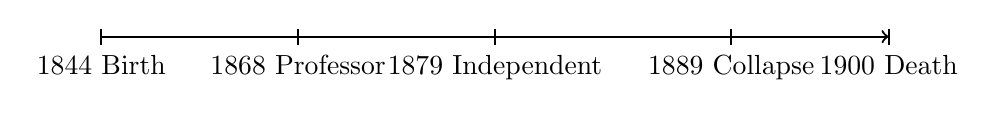
\begin{tikzpicture}
\draw[thick, ->] (0,0) -- (10,0);
\foreach \x/\label in {0/1844 Birth, 2.5/1868 Professor, 5/1879 Independent, 8/1889 Collapse, 10/1900 Death}
\draw[thick] (\x,0.1) -- (\x,-0.1) node[below] {\label};
\end{tikzpicture}
\end{center}
\end{frame}

\begin{frame}{Nietzsche's Writing Style: Provocative and Aphoristic}
\begin{itemize}
\item Nietzsche deliberately avoided writing systematic philosophical treatises, preferring a more literary approach.
\item He wrote in an \textbf{aphoristic style} - short, dense paragraphs expressing complete thoughts that reward careful reading.
\item His tone is often provocative, using hyperbole, metaphor, and shocking statements to challenge readers' assumptions.
\item Nietzsche wants to shake readers awake rather than merely present arguments for intellectual consideration.
\end{itemize}

\begin{exampleblock}{Example from \textit{Beyond Good and Evil}}
``Gradually it has become clear to me what every great philosophy has been: namely, the personal confession of its author and a kind of involuntary and unconscious memoir; also that the moral (or immoral) intentions in every philosophy constituted the real germ of life from which the whole plant has grown.''
\end{exampleblock}
\end{frame}


\begin{frame}{The Historical Context: Post-Enlightenment Europe}
\begin{itemize}
\item Nietzsche wrote during a time of significant cultural and intellectual transition in Europe, as traditional religious authority declined.
\item The rise of science, industrialization, and democratic movements were reshaping society and challenging old values.
\item The phrase \textbf{"God is dead"} captures Nietzsche's recognition that European culture was losing its religious foundations.
\item He saw both dangers and opportunities in this transition, warning of potential nihilism but also the chance for new values.
\end{itemize}

\begin{block}{Historical Influences}
\begin{itemize}
\item Ancient Greek culture (especially pre-Socratic philosophers)
\item German Romanticism and idealism
\item Arthur Schopenhauer's pessimism
\item Darwin's evolutionary theory
\end{itemize}
\end{block}
\end{frame}

\begin{frame}{Key Works in Nietzsche's Ethics}
\begin{itemize}
\item \textit{Human, All Too Human} (1878): Nietzsche's first work to directly criticize morality and religion.
\item \textit{The Gay Science} (1882): Introduces the "death of God" and eternal recurrence concepts.
\item \textit{Thus Spoke Zarathustra} (1883-1885): Fictional narrative presenting Nietzsche's most famous ideas.
\item \textit{On the Genealogy of Morality} (1887): His most sustained critique of conventional morality's historical development.
\end{itemize}

\begin{table}
\scriptsize
\begin{tabular}{ll}
\toprule
\textbf{Early Period} & Classical philology, influence of Wagner and Schopenhauer \\
\midrule
\textbf{Middle Period} & Break with earlier influences, focus on psychology and critique \\
\midrule
\textbf{Late Period} & Most influential ethical works, revaluation of values \\
\bottomrule
\end{tabular}
\end{table}
\end{frame}

\begin{frame}{What Makes Nietzsche's Ethics Different?}
\begin{itemize}
\item Unlike Kant or utilitarians, Nietzsche does not provide a systematic theory of right action or moral rules.
\item He offers a \textbf{critique of morality itself}, questioning its origin, value, and effects on human flourishing.
\item Nietzsche employs a \textbf{genealogical method}, examining how moral concepts developed historically rather than assuming their eternal truth.
\item His approach is descriptive and evaluative rather than prescriptive, focusing on psychological and cultural analysis.
\end{itemize}

\begin{center}
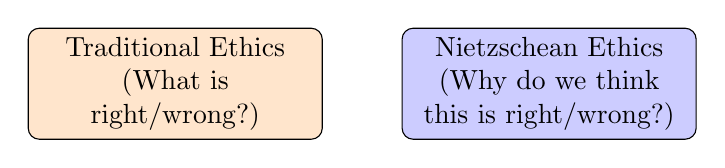
\begin{tikzpicture}
\node[draw, rectangle, rounded corners, fill=orange!20, text width=3.5cm, align=center] (a) {Traditional Ethics\\(What is right/wrong?)};
\node[draw, rectangle, rounded corners, fill=blue!20, text width=3.5cm, align=center, right=1cm of a] (b) {Nietzschean Ethics\\(Why do we think this is right/wrong?)};
\path[->] (a) -- (b);
\end{tikzpicture}
\end{center}
\end{frame}

\begin{frame}{Nietzsche's Big Question: What's Wrong with Morality?}
\begin{itemize}
\item Nietzsche asks: What if conventional morality is harmful to the flourishing of exceptional individuals?
\item He challenges us to reexamine our moral assumptions rather than just accepting them as given.
\item Morality might be useful for maintaining social order but could constrain human excellence and creativity.
\item His critique is not about rejecting all values but questioning whether our current values serve human flourishing.
\end{itemize}

\begin{alertblock}{Central Claim}
"What if a symptom of regression lurked in the 'good'... So that morality itself were to blame if the highest power and splendor possible to the type man was never in fact attained?" (GM Preface:6)
\end{alertblock}
\end{frame}

\begin{frame}{Understanding "Morality in the Pejorative Sense" (MPS)}
\begin{itemize}
\item Nietzsche doesn't criticize all forms of ethics or values, but targets what he calls \textbf{"morality in the pejorative sense"} (MPS).
\item MPS refers specifically to moral systems that claim universal authority and prioritize values like equality, altruism, and pity.
\item Examples of MPS include Christian morality, Kantian ethics, and utilitarianism, which all share certain problematic features.
\item Nietzsche believes these moralities emerged from particular historical and psychological conditions, not universal truths.
\end{itemize}

\begin{block}{Characteristics of MPS}
\begin{itemize}
\item Claims universal authority ("one morality for all")
\item Promotes selflessness, altruism, and equality
\item Devalues self-interest, ambition, and competition
\item Presents itself as objective and beyond questioning
\end{itemize}
\end{block}
\end{frame}
    
 
\begin{frame}{Descriptive vs. Normative Components of Morality}
\begin{itemize}
\item Nietzsche identifies two components in moral systems that he critiques separately.
\item The \textbf{descriptive component} consists of claims about human nature, agency, and psychology that morality presupposes.
\item The \textbf{normative component} consists of the specific values and judgments that a moral system promotes.
\item Both components are problematic for Nietzsche, but for different reasons.
\end{itemize}

\begin{table}
\centering
\begin{tabular}{|c|c|}
\hline
\textbf{Component} & \textbf{Description} \\
\hline
Descriptive Component & False claims about human nature \\
\hline
Normative Component & Harmful values for higher types \\
\hline
\end{tabular}
\caption{Components of Morality in the Pejorative Sense}
\end{table}   
\end{frame}

\begin{frame}{Critique \#1: The Problem with Free Will}
\begin{itemize}
\item Morality assumes that humans have \textbf{free will} - the ability to choose actions independently of causal determination.
\item Nietzsche rejects this, arguing that our choices are determined by unconscious psychological and physiological factors.
\item The idea that we are consciously "choosing" our actions is an illusion; our consciousness is largely epiphenomenal.
\item Without free will, moral responsibility (praise and blame) loses its foundation.
\end{itemize}

\begin{exampleblock}{Nietzsche's View}
"The 'inner world' is full of phantoms... The will no longer moves anything, hence does not explain anything either - it merely accompanies events; it can also be absent." (Twilight of the Idols)
\end{exampleblock}
\end{frame}

\begin{frame}{The "Doctrine of Types": How We're Shaped by Nature}
\begin{itemize}
\item Nietzsche proposes what scholars call the \textbf{"Doctrine of Types"} - the view that each person has a fixed psycho-physical constitution.
\item This constitution consists of unconscious drives, affects, and physiological factors that largely determine who we are.
\item Our conscious thoughts, values, and beliefs arise from these deeper type-facts rather than from rational deliberation.
\item Different human types flourish under different conditions, making universal moral prescriptions problematic.
\end{itemize}

\begin{alertblock}{Key Insight}
"Our moral judgments and evaluations... are only images and fantasies based on a physiological process unknown to us." (Daybreak 119)
\end{alertblock}
\end{frame}


\begin{frame}{Critique \#2: The Illusion of Self-Knowledge}
\begin{itemize}
\item Morality assumes we have \textbf{transparent self-knowledge} - that we know our true motives and can evaluate them.
\item Nietzsche argues that we have little access to our true motivations, which stem from unconscious drives.
\item He claims that "every action is unknowable" because we cannot access the totality of drives that determine our behavior.
\item Without self-transparency, moral systems that rank motives and intentions (like Kantian ethics) become problematic.
\end{itemize}

\begin{block}{The Iceberg Model of Mind}
\begin{center}
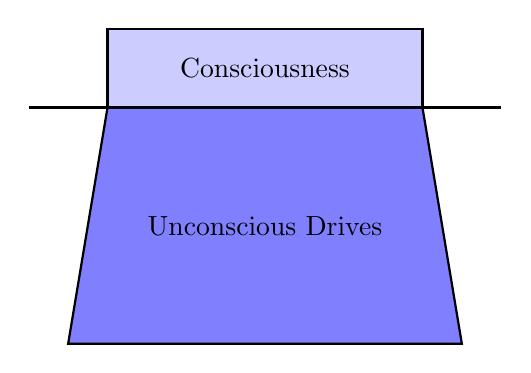
\begin{tikzpicture}
% Draw the top part (Consciousness)
\draw[thick, fill=blue!20] (-2,0) rectangle (2,1);
% Draw the submerged part (Unconscious Drives)
\draw[thick, fill=blue!50] (-2.5,-3) -- (2.5,-3) -- (2,0) -- (-2,0) -- cycle;
% Draw water line
\draw[thick] (-3,0) -- (3,0);
% Labels
\node at (0,0.5) {Consciousness};
\node at (0,-1.5) {Unconscious Drives};
\end{tikzpicture}
\end{center}
\end{block}

\end{frame}

\begin{frame}{Critique \#3: One Size Doesn't Fit All}
\begin{itemize}
\item Morality assumes that humans are \textbf{essentially similar} in relevant respects, so one moral code can apply to all.
\item Nietzsche argues that humans differ fundamentally in their drives, capacities, and conditions for flourishing.
\item What is good for one type of person may be harmful to another type's development and flourishing.
\item Universal morality wrongly treats all humans as if they have the same needs and potentials.
\end{itemize}

\begin{exampleblock}{The Cornaro Example}
Nietzsche describes how an Italian nobleman named Cornaro mistakenly believed that his slender diet was good for everyone, when in fact it only suited his particular physiology. Moralities make the same mistake in prescribing universal rules.
\end{exampleblock}
\end{frame}

\begin{frame}{The Slave Revolt in Morality}
\begin{itemize}
\item In \textit{On the Genealogy of Morality}, Nietzsche offers a historical account of how our current morality emerged.
\item He describes a \textbf{"slave revolt in morality"} where the socially weak revalued the values of the powerful.
\item Originally, "good" meant noble, powerful, and beautiful; "bad" simply meant base, common, or weak.
\item The slaves (particularly through Judaism and Christianity) inverted these values, making humility, meekness, and suffering "good" and power and strength "evil."
\end{itemize}

\begin{center}
\begin{tabular}{|c|c|}
\hline
\textbf{Master Morality} & \textbf{Slave Morality} \\
\hline
Good = Noble, Powerful & Good = Humble, Meek \\
Bad = Common, Weak & Evil = Proud, Strong \\
\hline
\end{tabular}
\end{center}
\end{frame}



\begin{frame}{Origins of Christian Morality: Ressentiment}
\begin{itemize}
\item The slave revolt in morality was motivated by \textbf{ressentiment} - a psychological state of repressed envy and hatred.
\item Unable to express their hostility directly, the powerless created moral values that condemned the powerful.
\item This "imaginative revenge" made a virtue of weakness and a sin of strength and self-affirmation.
\item The triumph of this morality represents "the victory of the weak over the strong" through conceptual means.
\end{itemize}

\begin{alertblock}{Creative Revaluation}
"The slave revolt in morality begins when ressentiment itself becomes creative and gives birth to values: the ressentiment of beings denied the true reaction, that of deed, who compensate with an imaginary revenge." (GM I:10)
\end{alertblock}
\end{frame}


\begin{frame}{What Nietzsche Rejects: Pity, Selflessness, and Equality}
\begin{itemize}
\item Nietzsche criticizes the central values of conventional morality as harmful to human excellence.
\item \textbf{Pity} (or compassion) keeps suffering alive rather than promoting true flourishing and enables a harmful focus on weakness.
\item \textbf{Selflessness} denies the importance of developing one's own capacities and projects, which are necessary for greatness.
\item \textbf{Equality} ignores natural differences between humans and treats as equal what is fundamentally unequal.
\end{itemize}

\begin{block}{Pro and Con Attitudes in MPS}
\begin{center}
\begin{tabular}{|c|c|}
\hline
\textbf{Pro} & \textbf{Con} \\
\hline
Happiness & Suffering \\
Altruism & Self-interest \\
Equality & Inequality \\
Pity & Indifference to suffering \\
\hline
\end{tabular}
\end{center}
\end{block}
\end{frame}

\begin{frame}{Modern Portrayals of Slave Morality}
    \begin{itemize}
    \item Modern fiction has many characters who embody \textbf{slave morality} through their transformation of weakness into virtue.
    \item These characters often present a public face of moral righteousness while harboring intense resentment toward those with power or talent.
    \item They create moral systems that elevate their own limitations as virtues, while condemning others' abilities as vices.
    \item Their stories frequently reveal the psychological complexity Nietzsche identified in the "slave revolt in morality."
    \end{itemize}
    
    \begin{center}
        \scriptsize
    \begin{tabular}{|p{3cm}|p{7cm}|}
    \hline
    \textbf{Character} & \textbf{Slave Morality Traits} \\
    \hline
    Dolores Umbridge (Harry Potter) & Uses "rules" and "order" to mask sadism; condemns others while enjoying her power \\
    \hline
    Cersei Lannister (Game of Thrones) & Transforms victimhood into vindictive morality; judges others for sins she commits \\
    \hline
    Chuck McGill (Better Call Saul) & Masks envy of his brother's talents as moral superiority and concern for legal ethics \\
    \hline
    Pete Campbell (Mad Men) & Resents Don's natural talents while claiming moral high ground through rule-following \\
    \hline
    Principal Rooney (Ferris Bueller) & Obsessed with punishing Ferris's freedom, disguising envy as concern for "rules" \\
    \hline
    \end{tabular}
    \end{center}
    \end{frame}


\begin{frame}{The Problem with Happiness as a Goal}
\begin{itemize}
\item Conventional morality promotes \textbf{happiness} (pleasure, comfort, contentment) as a primary good.
\item Nietzsche rejects this, claiming that the pursuit of happiness makes people "ridiculous and contemptible."
\item The higher human type is not defined by happiness but by creative achievement and overcoming challenges.
\item The "last men" who invented happiness are the "most despicable" in Nietzsche's view, content with comfort and safety.
\end{itemize}

\begin{exampleblock}{The Last Men}
"'What is love? What is creation? What is longing? What is a star?' thus asks the last man, and he blinks. The earth has become small, and on it hops the last man, who makes everything small... 'We have invented happiness,' say the last men, and they blink." (Thus Spoke Zarathustra)
\end{exampleblock}
\end{frame}

\begin{frame}{The Value of Suffering in Nietzsche's Ethics}
\begin{itemize}
\item While conventional morality aims to minimize suffering, Nietzsche sees \textbf{suffering as necessary} for human excellence.
\item Suffering creates depth, builds character, and enables genuine achievement and creativity.
\item The attempt to eliminate suffering through morality may prevent the conditions necessary for greatness.
\item This doesn't mean Nietzsche celebrates pointless suffering, but that he recognizes its transformative potential.
\end{itemize}

\begin{alertblock}{Key Insight}
"The discipline of suffering, of great suffering—do you not know that only this discipline has created all enhancements of man so far?" (Beyond Good and Evil 225)
\end{alertblock}
\end{frame}

\begin{frame}{"That Which Does Not Kill Me Makes Me Stronger"}
\begin{itemize}
\small
\item One of Nietzsche's most famous quotes captures his view that challenges strengthen us when overcome.
\item He argues that \textbf{resistance} and difficulty are necessary conditions for growth and achievement.
\item A life of ease and comfort leads to weakness, while overcoming obstacles creates excellence.
\item Nietzsche drew this insight partly from his own experience with severe physical illness and its effect on his thinking.
\end{itemize}
\begin{tikzpicture}[scale=0.6]
\scriptsize
\draw[thick] (0,-2) -- (10,-2); % Adjusted x-axis position
\draw[->] (0,-2) -- (0,4); % Adjusted y-axis position
\node[left] at (0,4) {Growth};
\node[below] at (10,-2) {Challenge/Suffering};

% Scatter plot points
\fill[blue] (2,0) circle (2pt) node[above right] {Low Growth};
\fill[blue] (8,3) circle (2pt) node[above right] {High Growth};

% Labels for overcoming and avoidance
\node[blue] at (7,4.0) {Overcoming};
\node[blue] at (2,-0.5) {Avoidance};
\end{tikzpicture}
\end{frame}

\begin{frame}{Nietzsche's Positive Vision: Beyond Good and Evil}
\begin{itemize}
\item Though known for his critiques, Nietzsche does offer a positive ethical vision centered on human excellence.
\item He envisions a \textbf{"revaluation of all values"} that moves beyond the framework of conventional morality.
\item This new valuation would promote the flourishing of exceptional individuals rather than the comfort of the majority.
\item Nietzsche's approach has been described as a form of "perfectionism" focused on human achievement and excellence.
\end{itemize}

\begin{block}{Beyond Good and Evil}
Moving "beyond good and evil" doesn't mean abandoning all values, but:
\begin{itemize}
\item Recognizing the historical origins of our moral concepts
\item Questioning universal applicability of moral rules
\item Creating values that enhance life and human potential
\item Evaluating morality by its effects on human flourishing
\end{itemize}
\end{block}
\end{frame}

\begin{frame}{The "Higher Human Being": What Nietzsche Values}
\begin{itemize}
\item Nietzsche's ethics centers on the cultivation and flourishing of \textbf{"higher human beings"} or "higher types."
\item His paradigmatic examples include creative geniuses like Goethe and Beethoven, who embodied human excellence.
\item These individuals express powerful creativity, independence of mind, and psychological complexity.
\item The worth of a culture or society is measured by its ability to produce and nurture such exceptional individuals.
\end{itemize}

\begin{exampleblock}{Exemplars of the Higher Type}
\begin{itemize}
\item Johann Wolfgang von Goethe (German poet and polymath)
\item Ludwig van Beethoven (German composer)
\item Napoleon Bonaparte (French military and political leader)
\item Nietzsche himself (in his self-assessment)
\end{itemize}
\end{exampleblock}
\end{frame}

\begin{frame}{Traits of Higher Types: Solitude and Self-Sufficiency}
\begin{itemize}
\item Higher types exhibit distinctive characteristics that differentiate them from the "herd."
\item They value \textbf{solitude} and independence, avoiding the crowds and conventional opinion.
\item They show \textbf{self-reverence}, possessing a fundamental certainty about themselves and their values.
\item They embrace life-affirming attitudes, accepting both pleasure and suffering as part of a complete life.
\end{itemize}

\begin{alertblock}{Five Key Characteristics of Higher Types}
\begin{enumerate}
\item Solitude and independence
\item Pursuit of a unifying creative project
\item Psychological health and resilience
\item Life-affirmation (willing eternal recurrence)
\item Self-reverence rather than self-doubt
\end{enumerate}
\end{alertblock}
\end{frame}

\begin{frame}{Batman: The Higher Type and Self-Creation}
    \begin{itemize}
    \item Batman exemplifies Nietzsche's \textbf{higher type} by transforming personal tragedy into creative purpose.
    \item He creates his own moral framework outside conventional justice systems—an example of "revaluation of values."
    \item His solitude, self-discipline, and single-minded focus reflect Nietzschean virtues of the exceptional individual.
    \item Batman's ongoing struggle with whether to kill (especially the Joker) represents the tension between creating new values and being bound by old ones.
    \end{itemize}
    
    \begin{exampleblock}{Nietzschean Traits in Batman}
    Batman demonstrates central Nietzschean virtues: he creates meaning from suffering, values self-mastery over comfort, stands apart from herd thinking, and imposes his vision on the world through sheer will. However, his rigid adherence to not killing may represent the lingering influence of conventional morality Nietzsche critiqued.
    \end{exampleblock}
    \end{frame}

\begin{frame}{The Joker: A Misreading of Nietzsche's Critique}
    \begin{itemize}
    \item The Joker (especially in \textit{The Dark Knight}) is often misinterpreted as embodying Nietzschean values by rejecting conventional morality.
    \item However, the Joker represents nihilism—the absence of all values—which Nietzsche sought to overcome, not promote.
    \item While he claims to expose the hypocrisy of society's morals, the Joker offers no affirmative values or life-enhancing alternative.
    \item His destructiveness and chaos reflect \textbf{passive nihilism}, not the active creation of new values that Nietzsche advocated.
    \end{itemize}
    
    \begin{alertblock}{Common Misinterpretation}
    The Joker's "beyond good and evil" stance is a dangerous caricature of Nietzsche's thought. Nietzsche didn't advocate destroying all values, but replacing harmful values with life-affirming ones. The Joker's celebration of meaninglessness is precisely what Nietzsche feared would follow the "death of God" if new values weren't created.
    \end{alertblock}
    \end{frame}


\begin{frame}{Creative Geniuses as Nietzsche's Ideal}
\begin{itemize}
\item The traits Nietzsche values are particularly evident in creative geniuses and artistic innovators.
\item \textbf{Creative individuals} demonstrate the capacity to overcome convention and create new values.
\item Their willingness to stand apart from society and endure hardship enables unique achievements.
\item "The men of great creativity... are the really great men according to my understanding." (WP 957)
\end{itemize}

\begin{center}
\begin{tabular}{ccc}
& Life-affirmation & \\
& $\downarrow$ & \\
Solitude $\rightarrow$ & \fbox{Creative Genius} & $\leftarrow$ Self-sufficiency \\
& $\uparrow$ & \\
& Resilience & \\
\end{tabular}
\end{center}
\end{frame}


\begin{frame}{The Will to Power: Commonly Misunderstood}
\begin{itemize}
\item The concept of \textbf{will to power} is frequently misinterpreted as simple domination or political control.
\item For Nietzsche, it primarily describes a psychological drive for overcoming resistance and achieving mastery.
\item Will to power expresses itself in creativity, self-discipline, and the ability to transform oneself.
\item It is less a metaphysical doctrine about reality and more a psychological insight about human motivation.
\end{itemize}

\begin{block}{Two Key Interpretations of Will to Power}
\begin{itemize}
\item \textbf{Psychological}: A descriptive claim about human motivation and drives
\item \textbf{Evaluative}: A criterion for assessing values and actions based on whether they enhance power
\end{itemize}
\end{block}
\end{frame}

\begin{frame}{Walter White: Ressentiment and Will to Power}
    \begin{itemize}
    \item Walter White's transformation in \textit{Breaking Bad} begins with classic \textbf{ressentiment}—resentful awareness of his unrealized potential.
    \item His initial motivation (providing for his family) gradually reveals itself as a mask for his true drive for power, recognition, and excellence.
    \item White's famous declaration "I am the one who knocks" marks his rejection of his former slave morality position.
    \item His trajectory shows both creative self-overcoming and destructive hubris, illustrating the danger of will to power without ethical constraints.
    \end{itemize}
    
    \begin{block}{The Danger of Misunderstood Will to Power}
    Walt's journey demonstrates how Nietzsche's concepts can be dangerously misapplied when "will to power" is understood merely as domination rather than creative self-mastery. His transformation embodies both the exhilaration of breaking free from conventional constraints and the tragedy of unchecked ambition divorced from life-affirming values.
    \end{block}
    \end{frame}

\begin{frame}{Perspectivism: No Objective Moral Facts}
\begin{itemize}
\small
\item Nietzsche's \textbf{perspectivism} holds that there is no single, objective viewpoint on the world, only perspectives.
\item In ethics, this means there are no objective moral facts, only different moral perspectives.
\item Values don't exist "in themselves" but are created through human valuation and interpretation.
\end{itemize}

\begin{center}
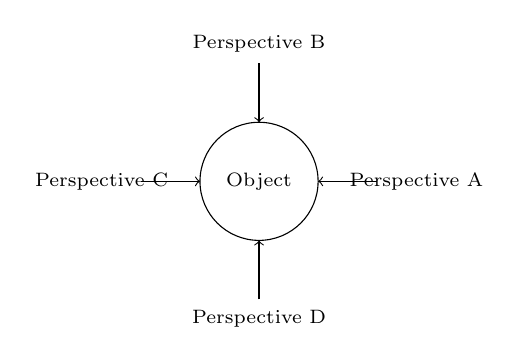
\begin{tikzpicture}[scale = 0.5]
\scriptsize
\draw (0,0) circle (1.5cm);
\node at (0,0) {Object};

\draw[->] (3,0) -- (1.5,0);
\node at (4,0) {Perspective A};

\draw[->] (0,3) -- (0,1.5);
\node at (0,3.5) {Perspective B};

\draw[->] (-3,0) -- (-1.5,0);
\node at (-4,0) {Perspective C};

\draw[->] (0,-3) -- (0,-1.5);
\node at (0,-3.5) {Perspective D};
\end{tikzpicture}
\end{center}
\end{frame}

\begin{frame}{Is Nietzsche a Relativist?}
\begin{itemize}
\item Nietzsche's anti-realism about values raises the question: is he simply a moral relativist?
\item He rejects the view that all moral perspectives are equally valid or that any moral view is as good as any other.
\item He maintains that some values better serve human flourishing and excellence than others.
\item Nietzsche's position is better described as \textbf{moral anti-realism} combined with a perfectionist ethic.
\end{itemize}

\begin{exampleblock}{Nietzsche on Relativism}
"It is not error as error that" he fundamentally objects to in morality (EH IV:7). The problem isn't that morality is false in some objective sense, but that it is harmful to the flourishing of higher types.
\end{exampleblock}
\end{frame}

\begin{frame}{"God is Dead": Moral Implications}
\begin{itemize}
\item Nietzsche's famous pronouncement that \textbf{"God is dead"} has profound implications for morality.
\item Without a divine lawgiver or transcendent order, traditional morality loses its metaphysical foundation.
\item This creates both a crisis (nihilism) and an opportunity (freedom to create new values).
\item The death of God requires humans to take responsibility for creating meaning and values themselves.
\end{itemize}

\begin{alertblock}{The Madman's Pronouncement}
"God is dead. God remains dead. And we have killed him... What water is there for us to clean ourselves? What festivals of atonement, what sacred games shall we have to invent?" (The Gay Science 125)
\end{alertblock}
\end{frame}


\begin{frame}{The Eternal Recurrence as an Ethical Test}
\begin{itemize}
\item The \textbf{eternal recurrence} is Nietzsche's thought experiment about affirming life in its totality.
\item It asks: What if you had to live your exact life over and over again for eternity, with every pain and joy repeated?
\item Those who can embrace this prospect demonstrate the highest affirmation of life possible.
\item The eternal recurrence functions as an ethical test rather than a metaphysical doctrine.
\end{itemize}

\begin{exampleblock}{The Greatest Weight}
    \small
"What, if some day or night a demon were to steal after you into your loneliest loneliness and say to you: 'This life as you now live it and have lived it, you will have to live once more and innumerable times more'... Would you not throw yourself down and gnash your teeth and curse the demon who spoke thus? Or have you once experienced a tremendous moment when you would have answered him: 'You are a god and never have I heard anything more divine.'" (GS 341)
\end{exampleblock}
\end{frame}

\begin{frame}{Severus Snape: Eternal Recurrence and Life Affirmation}
    \begin{itemize}
    \item Snape's life choices present an interesting test case for Nietzsche's idea of \textbf{eternal recurrence}.
    \item His life contains immense suffering: childhood poverty, bullying, unrequited love, and living as a double agent.
    \item Yet Snape never rejects his path, continuing to protect Harry out of love for Lily, affirming his choices despite their cost.
    \item When dying, Snape doesn't express regret but gives Harry his memories—symbolically accepting his life's meaning.
    \end{itemize}
    
    \begin{alertblock}{Affirmation Through Suffering}
    Would Snape will the eternal recurrence of his life with all its pain? His final actions suggest he might—he doesn't seek to erase his suffering but gives it meaning through his protection of Harry. This exemplifies Nietzsche's view that the highest affirmation includes embracing even life's painful aspects.
    \end{alertblock}
    \end{frame}

\begin{frame}{Becoming Who You Are: Self-Creation within Constraints}
\begin{itemize}
\item Nietzsche's famous imperative \textbf{"become who you are"} captures his view of authentic self-development.
\item This is not unlimited self-creation, as we are constrained by our natural type and physiological constitution.
\item Self-creation happens within these constraints, through recognizing and cultivating one's distinctive qualities.
\item "One becomes what one is" through self-discipline, affirming necessity, and developing one's unique potential.
\end{itemize}

\begin{block}{The Paradox of Self-Creation}
\begin{itemize}
\item We cannot choose our fundamental drives and capacities
\item Yet we can shape how these drives express themselves
\item Self-knowledge means recognizing our limitations
\item "Freedom" is accepting necessity while developing our potential
\end{itemize}
\end{block}
\end{frame}

\begin{frame}{Nietzsche's Critique of Democracy and Equality}
\begin{itemize}
\item Nietzsche is highly critical of democratic movements and egalitarian politics of his time.
\item He sees \textbf{democratic values} as expressions of herd mentality that level down excellence to mediocrity.
\item Modern politics, in his view, secularizes Christian morality's emphasis on equality and care for the weak.
\item The elevation of the "common man" threatens the conditions necessary for the cultivation of greatness.
\end{itemize}

\begin{alertblock}{A Challenging Perspective}
"The democratic movement is the heir of the Christian movement." (BGE 202)

"Every elevation of the type 'man' has so far been the work of an aristocratic society." (BGE 257) 
\end{alertblock}
\end{frame}

\begin{frame}{Is Nietzsche Political? Common Misconceptions}
\begin{itemize}
\item Despite his cultural critiques, Nietzsche does not present a systematic \textbf{political philosophy}.
\item His primary concern is cultural and individual transformation, not political structures or systems.
\item He expresses hostility toward politics, calling the state "the coldest of all cold monsters."
\item Nietzsche functions more as an "esoteric moralist" addressing select individuals rather than advocating political change.
\end{itemize}

\begin{table}
\begin{tabular}{ll}
\toprule
\textbf{Misconception} & \textbf{Nietzsche's Actual View} \\
\midrule
Advocate for aristocratic politics & Critic of all political systems \\
Proto-fascist thinker & Despised nationalism and antisemitism \\
Political revolutionary & Focused on individual transformation \\
Systematic political theorist & No developed political philosophy \\
\bottomrule
\end{tabular}
\end{table}
\end{frame}

\begin{frame}{Nietzsche's Legacy in 20th Century Ethics}
    \begin{itemize}
    \item Nietzsche's influence extends far beyond academic philosophy to psychology, literature, and culture.
    \item \textbf{Existentialist thinkers} like Sartre and Camus developed his insights about meaning in a godless world.
    \item Postmodern philosophers such as Foucault expanded his genealogical approach to exploring power and knowledge.
    \item Feminist philosophers have both critiqued his apparent misogyny and adapted his critique of moral systems.
    \end{itemize}
    
    \begin{block}{Major Philosophical Inheritors}
    \begin{itemize}
    \item Max Weber (sociology of value and meaning)
    \item Martin Heidegger (authenticity and critique of modernity)
    \item Michel Foucault (genealogy and power analysis)
    \item Bernard Williams (critique of "morality system")
    \end{itemize}
    \end{block}
    \end{frame}
    
    \begin{frame}{Common Criticisms of Nietzsche's Ethics}
    \begin{itemize}
    \item Critics argue that Nietzsche's \textbf{elitism} and rejection of equality undermine his ethical vision.
    \item His emphasis on exceptional individuals seems to neglect the welfare of ordinary people.
    \item His critique of compassion appears callous and potentially justifies indifference to suffering.
    \item His rejection of universal moral principles could lead to dangerous moral relativism.
    \end{itemize}
    
    \begin{center}
        \small
    \begin{tabular}{|p{5cm}|p{5cm}|}
    \hline
    \textbf{Criticism} & \textbf{Possible Response} \\
    \hline
    Dangerous elitism & Focus on excellence, not political hierarchy \\
    \hline
    Disregard for ordinary people & Cultural flourishing benefits all indirectly \\
    \hline
    Rejection of compassion seems cruel & Critiques ineffective compassion, not all care \\
    \hline
    Leads to moral relativism & Offers positive values, not "anything goes" \\
    \hline
    \end{tabular}
    \end{center}
    \end{frame}
    
       
    \begin{frame}{Conclusion: Nietzsche's Challenge to Conventional Ethics}
    \begin{itemize}
    \item Nietzsche offers a profound challenge to our moral assumptions, asking us to examine their origins and effects.
    \item His critique encourages us to question whether conventional morality truly supports human flourishing and excellence.
    \item While rejecting universal moral systems, Nietzsche affirms the importance of creating values that enhance life.
    \item His philosophy invites us to honestly confront difficult questions about what kind of life is truly worth living.
    \end{itemize}
    
    \begin{alertblock}{Nietzsche's Enduring Questions}
    \begin{itemize}
    \item What values truly enhance human flourishing?
    \item How might conventional morality constrain excellence?
    \item What would it mean to create values beyond good and evil?
    \item How can we affirm life in all its complexity?
    \end{itemize}
    \end{alertblock}
    
    \end{frame}

\end{document}